\documentclass{article}

% if you need to pass options to natbib, use, e.g.:
%     \PassOptionsToPackage{numbers, compress}{natbib}
% before loading neurips_2019

% ready for submission
% \usepackage{neurips_2019}

% to compile a preprint version, e.g., for submission to arXiv, add add the
% [preprint] option:
%     \usepackage[preprint]{neurips_2019}

% to compile a camera-ready version, add the [final] option, e.g.:
\usepackage[]{neurips_2019}

% to avoid loading the natbib package, add option nonatbib:
%     \usepackage[nonatbib]{neurips_2019}

\usepackage[utf8]{inputenc} % allow utf-8 input
\usepackage[T1]{fontenc}    % use 8-bit T1 fonts
\usepackage{hyperref}       % hyperlinks
\usepackage{url}            % simple URL typesetting
\usepackage{booktabs}       % professional-quality tables
\usepackage{amsfonts}       % blackboard math symbols
\usepackage{nicefrac}       % compact symbols for 1/2, etc.
\usepackage{microtype}      % microtypography
\usepackage{graphicx}
\graphicspath{{./images/}}

\title{Math189 Midterm Report: Instrument Recognition Through Machine Learning}

\begin{document}

\maketitle

\begin{abstract}
  Automated instrument recognition a desirable task within the The music information retrieval (MIR) field. Although humans are relatively adept at distinguishing between instruments, a robust Artificial intelligence system would provide valuable application purposes. Through the use of Machine learning algorithms, such as Random Forest, we that can identify the instrument being played in a monophonic audio track. To temporarily narrow the scope of this project, the model has been limited to 10 musical instruments and inputs are single notes.
\end{abstract}

\section{Introduction}

Music is most often created through a combination of instruments and vocals. With adequate exposure, a human can usually identify common instruments that are used in a music; However, due to stylistic differences between artists and the quality differences between recordings, it is still difficult for computers automatically recognize individual instruments.

In the current digitized world, music is highly accessible through the internet and various streaming platforms. The high availability of recordings makes instrument recognition a desirable task within the The music information retrieval (MIR) field. The ability to automate instrument recognition will allow for processes commonly used in music related platforms, such as genre classification and song recommendation, to be improved.

The goal of this project is to create a machine learning model that can identify the instrument being played in a monophonic audio track. To temporarily narrow the scope of this project, the model has been limited to 10 musical instruments and inputs are single notes.

\section{Dataset}
\label{Dataset}

The dataset being used by this project is called the Nsynth Dataset provided by Magenta, an open source Python library. NSynth contains 305,979 musical notes with each audio file having a unique pitch, timbre, and envelope. These samples are annotated based on a both human evaluation and heuristic algorithms and contains information on the following:

\begin{itemize}
\item Source: Contains be labeled acoustic, electronic, or synthetic based on the method of sound production for the audio clip. Each note is labeled with a single source.
\item Family: Contain the labels bass, brass, flute, guitar, keyboard, mallet, organ, reed, string, synth lead, vocal. This indicated the high-level family of the instrument being played and each note is labeled with a single family. Due to a low number of samples, synth lead was discarded from the dataset.
\item Qualities: Contains the labels bright, dark, distortion, fast decay, long release, multiphonic, nonlinear env, percussive, reverb, and tempo-synced. These labels are given based on the sonic qualities of the note and each note is annotated with zero or more qualities.
\end{itemize}

For the purposes of this model, the "family" of each note is used to determine the instrument.

The dataset is split into three sets: train, test, and validation. A count of files within each set is given below in Table 1.

\begin{table}[htb]
  \caption{Nsynth Dataset Breakdown}
  \label{Nsynth-Dataset}
  \centering
  \begin{tabular}{lll}
    \toprule
    Set name & Sample Number \\
    \midrule
    Train & 289,205\\
    Test & 12,678 \\
    Validation & 4,096\\
    \bottomrule
  \end{tabular}
\end{table}

For the training of the current model, the actual training dataset was too large to handle with the current set up and therefore only the "validation" set was used. A detailed breakdown of the dataset is shown in figure 1.

\begin{figure}[htb]
  \centering
  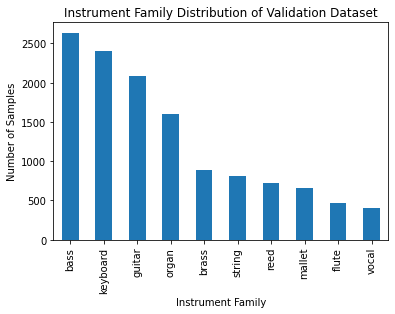
\includegraphics[width=.5\linewidth]{validation_dataset}
  \caption{Validation Data Set Distribution}
\end{figure}

\section{Audio Features}
\label{features}

In order to better represent the musical samples as data points for the model. Various features where extracted and used from each sample rather than the raw audio. The current features being used are listed and explained below.

\subsection{Mel Spectrogram}
A spectrogram is an intensity plot of the Short-Time Fourier Transform (STFT) magnitude. The spectrogram used for the model was adjusted to the mel scale, which represents pitches judged by listeners to be equal in distance one from another.

\subsection{Mel-Frequency Cepstral Coefficient (MFCC)}
The Mel-Frequency Cepstrum is found by spacing the frequency bands of the spectrum of a signal equally along the mel scale, and then taking the Fourier transform of the logarithm of the spectrum. The coefficients of this transformation represent the power spectrum of the signal

\subsection{Chroma}
The chroma of a signal is extracted by casting an audio signal into 12 semitones (chromas) based on their pitch within the musical octave. 
These features loses information regarding the absolute frequency of the signal but is useful in identifying relation between chroma of the audio signal.

\subsection{Spectral Contrast}
Spectral contrast is a measure of the difference in the spectral peak and the spectral valley in each frequency subband.

\subsection{Spectral Rolloff}
The spectral roll-off is determined by the frequency at each frame below which ${85}\%$  of the energy in the spectrogram is contained. The feature is used to differentiate sounds with different energy distributions. 

\subsection{Spectral Centroid}
Spectral centroid is determined by the mean of each frame in the spectrogram after its magnitude has been normalized.

\subsubsection{Zero-Cross Rating}
The zero-Cross rate is determined by the rate of sign-changes in an audio time series. The rate is found to be higher for noisy audio and audio that includes higher frequency signals.

\subsection{Harmonic/Percussive}
Harmonic sounds are perceived as pitched sound (eg. melodies, chords) where as percussive sound are noise-like and usually stems from instrument onsets (eg. hit on a drum, consonants in speech). The Harmonic/Percussive feature uses the ratio of harmonic to percussive sounds to classify whether the sound is more harmonic or more percussive.

\section{Model}

In order to train the instrument recognition model, a few different machine learning models where implemented, including: Random forest, Support-vector machine, Bayesian, and Principal Component analysis. From initial results, the accuracy of the Random forest algorithm was the best and therefore it was used as the final model.

\section{System Design}
\label{system}

The overall model is split into three sections: 
\begin{itemize}
    \item Database Branch: Takes in the training dataset, constructs a database of the associated features, and uses these features to inform the model
    \item Query Branch: Takes in an input audio file by the user. The query branch extracts the relevant feature of the query file, referred to as the query features, and passes it to the model for prediction.
    \item Output Branch: Currently presents the output of the model. An ensemble step may be included in the future if multiple models provide good results in recognizing different instruments.
\end{itemize}

A block diagram of the system is shown in figure 2.

\begin{figure}[htb]
  \centering
  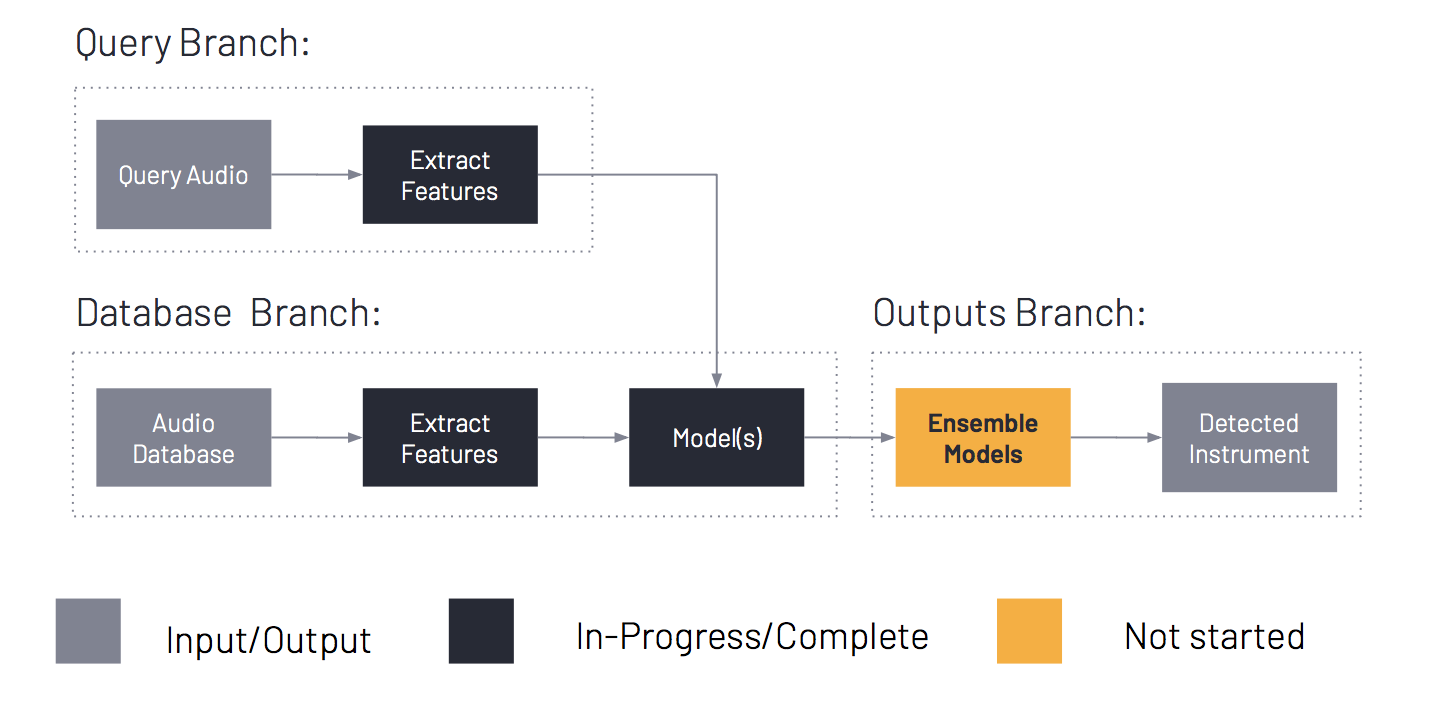
\includegraphics[width=1\linewidth]{system}
  \caption{System overview}
\end{figure}

\section{Initial Results}
\label{Results}

Due to the large amount of data in the dataset and number of features being extracted, the processing speed of the audio samples is relatively slow. In order to obtain initial results and quickly tune parameters to optimize the system, slight adjustments to the system were made. In the model used to get the following results, only features 3.1-3.3 were used in the feature extraction process and only a subsets of the validation dataset was used for both training and testing.

\subsection{Data Subset Used}
Since the validation dataset is relatively unbalance, as seen in figure 1, and requires a long time to process, a subset of the entire database was selected. The resulting dataset included 400 samples from each instrument family as shown in figure 3.

\begin{figure}[htb]
  \centering
  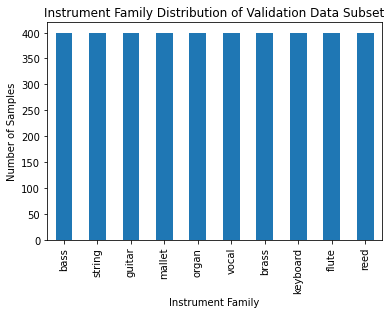
\includegraphics[width=.5\linewidth]{validation_subset}
  \caption{Validation Data Subset Distribution}
\end{figure}

This set of samples was then split into train and test sets, with a test size of $25\%$, resulting in 3000 training samples (300 from each instrument family) and 1000 test samples (100 from each instrument family) as shown in figure 4.

\begin{figure}[htb]
  \centering
  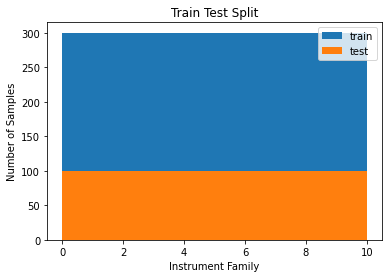
\includegraphics[width=.5\linewidth]{train_test_split}
  \caption{Data Train Test Split}
\end{figure}

\subsection{Output}
The results of the system is used to generate the following normalized confusion matrix:

\begin{figure}[htb]
  \centering
  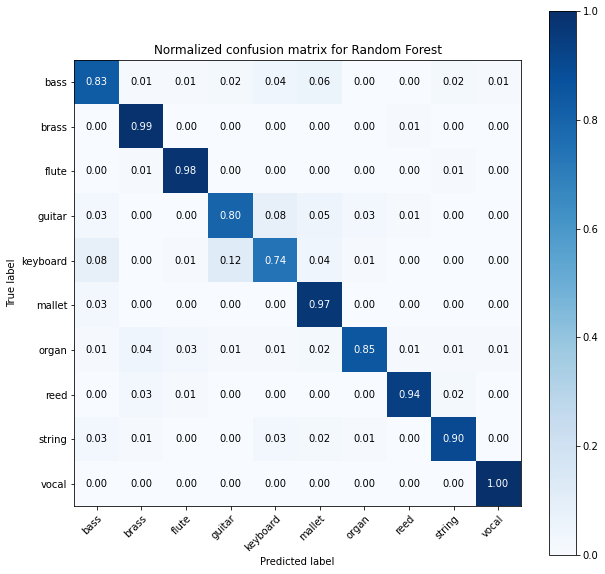
\includegraphics[width=.7\linewidth]{confusion_matrix}
  \caption{Output of the Random Forest Model}
\end{figure}

This confusion matrix illustrates a relatively high performance across all types of instrument recognition, a further breakdown of the results are detailed in table 2. 

\begin{table}[htb]
  \caption{Model Results Breakdown (Ordered by Descending Accuracy)}
  \label{results-table}
  \centering
  \begin{tabular}{ccccc}
    \toprule
    Instrument & accuracy & precision & recall & f1-score  \\
    \midrule
    vocal & 1.00 & 0.98 & 1.00 & 0.99\\
    brass & 0.99 & 0.91 & 0.99 & 0.95\\
    flute & 0.98 & 0.94 & 0.98 & 0.96\\
    mallet & 0.97 & 0.84 & 0.97 & 0.90\\
    reed & 0.94 & 0.97 & 0.94 & 0.95\\
    string & 0.90 & 0.94 & 0.90 & 0.92\\
    organ & 0.85 & 0.94 & 0.85 & 0.89\\
    bass & 0.83 & 0.82 & 0.83 & 0.83\\
    guitar & 0.80 & 0.84 & 0.80 & 0.82\\
    keyboard & 0.74 & 0.82 & 0.74 & 0.78\\
    \bottomrule
  \end{tabular}
\end{table}

These results show an accuracy range of $74.00\%-100.00\%$ and a f1-score range of $78.00\%-99.00\%$, which the accuracy being a relative predictor for f1-score performance. The overall accuracy of the model comes out to be $90.00\%$.

\section{Discussion}

From the accuracy and f1-scores, the overall performance of the model seems fairly good. There are some nuances that the model is specifically poor at distinguishing; for example, $12.00\%$ of the keyboard samples are incorrectly classified as guitar while $8.00\%$ of the guitar samples are incorrectly classified as keyboard, therefore suggesting that guitar and keyboard are particularly similar in terms of features. The most basic solution to this issue is to expand the data set, which is currently limited to shorten run time,so that the model sensitivity and specificity can be improved.

Some possible sources of error may come from the use of the dataset itself. In the dataset, there seems to be faulty samples which are silent, poorly recorded, or have been corrupted during conversion, therefor inaccurately informing the model. Additionally,the sources of the samples are differentiated as acoustic, electronic, and synthesized. These different types of sources may fundamentally differ in audio signatures and introduce unaccounted variables within the sample set.

Additional error may come from the feature extraction and model training process. The current audio features being used were selected based off of intuition, experience, and literature review. Although these features seem effective to an extent, there has been no metric implemented to show how effective each feature actually is, thus some features may actually be decreasing the performance of the model. Similarly, random forest was selected based on it's relatively good initial results. However, there was not rigorous testing done using other models, therefore random forest may not be the ideal system for this problem.

\section{Future work}

Some next steps for this project are outlined below. While sections 8.1 and 8.2 (Model Improvements and the Deep learning approach ) are expected to be implemented, sections 8.3 will be regarded as a stretch goal for this project.

\subsection{Model Improvement}
As mentioned in section 7 (Discussion) there are some improvements to be made in the prepossessing feature extraction steps. The prepossessing step should be be modified to discard faulty samples. While these faulty samples are easily distinguishable by ear, due large amounts of sample, an automated process is ideal. Additionally, all of the audio features extracted from the samples should be evaluate such that unimportant featured can be discarded.

Additional models may be tested for performance, and a grid search should be used to optimise parameter. If multiple models show promising results, an ensemble step will be included to combine the performance of each model.

\subsection{Deep Learning Approach}

While the current approach to this project has avoided deep learning techniques. Some literature review suggests that the most frequent approach to this problem has been to utilize convolutional neural networks (CNN), therefor a CNN may be implemented for comparison purposes

\subsection{Polyphonic Music Processing}
Currently the scope of the project is narrowed to single instrument audio clips, however, an interesting extension to this problem may be to classify multiple instruments within a single, polyphonic, audio clip.

\subsubsection*{Acknowledgments}

I would like to thank Prof. Gu and Siddarth for their support and
feedback throughout the the project development
process.

%\section*{References}

\end{document}
